\documentclass[11pt]{article}
\usepackage{amsmath}
\usepackage{booktabs}
\usepackage{multirow}

% added for table
\usepackage{longtable}
\usepackage{array}

\usepackage{MyTemplate}
\usepackage{fontspec}
\usepackage{amssymb}

% foot note
\usepackage[stable]{footmisc}

\begin{document}
% \newcommand{\adversarialexamples}{نمونه‌های مقابله‌ای}
\newcommand{\neuralnetwork}{شبکه‌های عصبی} 
\newcommand{\deepnetwork}{شبکه‌های عصبی ژرف}
\newcommand{\robustness}{مقاومت شبکه}
\newcommand{\attack}{حمله}









\newcommand{\hyperparameter}{ابرپارامتر}
\newcommand{\perturbation}{اختلال}
% \newcommand{\robustness}{استحکام}
\newcommand{\adversarialtraining}{آموزش خصمانه}
\newcommand{\freeadversarialtraining}{آموزش خصمانه‌ی رایگان}
\newcommand{\fastadversarialtraining}{آموزش خصمانه‌ی سریع}
\newcommand{\stepsize}{اندازه‌ی گام}
\newcommand{\curvature}{انحنا}

\newcommand{\robustnessaccuracytradeoff}{بده‌بستان دقت مستحکم-تمیز}
\newcommand{\clipping}{برش}
\newcommand{\secondorderoptimization}{بهینه‌سازی مرتبه دوم}
\newcommand{\catastrophicoverfitting}{بیش‌برازش فاجعه‌بار}

\newcommand{\backpropagation}{پس‌انتشار}

\newcommand{\lossfunction}{تابع زیان}
\newcommand{\projection}{تصویر}
\newcommand{\generalization}{تعمیم}
\newcommand{\singlestep}{تک‌مرحله‌ای}

\newcommand{\losslandscape}{چشم‌انداز تابع زیان}
\newcommand{\multistep}{چندمرحله‌ای}

\newcommand{\adversarialattack}{حمله‌ی خصمانه}

\newcommand{\locallinearity}{خطی‌بودن محلی}

\newcommand{\classifier}{دسته‌بند}
\newcommand{\robustaccuracy}{دقت مستحکم}
\newcommand{\epoch}{دوره}

\newcommand{\fastgradientsignmethod}{روش علامت گرادیان سریع}

\newcommand{\deepneuralnetwork}{شبکه‌ی عصبی ژرف}
\newcommand{\randomstart}{شروع تصادفی}

\newcommand{\projectedgradientdescent}{فرود گرادیان تصویرشده}

\newcommand{\minmax}{کمینه‌بیشینه}

\newcommand{\gradient}{گرادیان}

\newcommand{\adversarialexample}{مثال خصمانه}
\newcommand{\dataset}{مجموعه‌داده}
\newcommand{\architecture}{معماری}
\newcommand{\regularization}{منظم‌سازی}

\newcommand{\abnormaladversarialexample}{نمونه‌ی خصمانه‌ی نابهنجار}

\newcommand{\hessian}{هسی}
\newcommand{\gradientalignment}{هم‌راستایی گرادیان}
\thispagestyle{empty}
% \settextfont[Scale=1.2]{B_Nazanin.TTF}
\settextfont[
    Path=fonts/,
    UprightFont=BNazanin-Regular.ttf,
    BoldFont=BNazanin-Bold.ttf,
    Scale=1.2,
]{}
\begin{center}
\includegraphics{logo}
\vskip 1cm
{\bf
دانشگاه صنعتی شریف\\ دانشکده مهندسی کامپیوتر\\ سمینار کارشناسی ارشد گرایش هوش مصنوعی و رباتیکز\\
\vskip 1cm
عنوان:\\
% پیش‌بینی بیش‌برازش فاجعه‌بار در آموزش تخاصمی سریع\\
پیش‌بینی بیش‌برازش فاجعه‌بار در آموزش دشمنانه سریع\\
\lr{Predicting Catastrophic Overfitting in Fast Adversarial Training}
\vskip 1cm
نگارش:\\
فرزان رحمانی\\
403210725\\
\vskip 1cm
استاد راهنما:\\
دکتر محمدحسین رهبان\\
\vskip 1cm
استاد ممتحن داخلی:\\
دکتر شهره كسائی\\

\vskip 3.5cm

}
تیر ۱۴۰۵
\newpage
\end{center}



% \settextfont{B_Nazanin.TTF}
% \settextfont{B Nazanin}
% \settextfont[
%     Path=fonts/,
%     UprightFont=BNazanin-Regular.ttf,
%     BoldFont=BNazanin-Bold.ttf,
% ]{}
%\setdigitfont[Scale=1]{XB_Roya.ttf}[ItalicFont={XB_RoyaIt.ttf},BoldItalicFont={XB_RoyaBdIt.ttf}, BoldFont={XB_RoyaBd.ttf}]
\renewcommand{\labelitemi}{$\bullet$}


% {\bf {چکيده: }}
% شبکه‌های عصبی ژرف\LTRfootnote{\lr{Deep Neural Network}} در سال‌های اخیر در طیف گسترده‌ای از کاربردها به موفقیت‌های چشمگیری دست یافته‌اند،
% اما در برابر حملات دشمنانه\LTRfootnote{\lr{Adversarial Attacks}} بسیار آسیب‌پذیرند؛
% آشفتگی‌هایی\LTRfootnote{\lr{Perturbation}} کوچک و معمولاً نامحسوس که می‌توانند خروجی مدل را با اطمینان بالا نادرست کنند.
% آموزش دشمنانه\LTRfootnote{\lr{Adversarial Training}} یکی از مؤثرترین دفاع‌ها در برابر این حملات است،
% اما نسخه‌های چندمرحله‌ای\LTRfootnote{\lr{Multi-Step}} آن مانند روش مبتنی بر فرود گرادیان افکنش‌شده\LTRfootnote{\lr{Projected Gradient Descent}}
% از نظر محاسباتی پرهزینه‌اند.
% آموزش دشمنانه سریع\LTRfootnote{\lr{Fast Adversarial Training}} با استفاده از حملات تک‌مرحله‌ای\LTRfootnote{\lr{Single-Step}} مانند
% روش علامت گرادیان سریع\LTRfootnote{\lr{Fast Gradient Sign Method}} این هزینه را کاهش می‌دهد،
% اما با پدیده‌ای به نام بیش‌برازش فاجعه‌بار\LTRfootnote{\lr{Catastrophic Overfitting}} روبه‌روست؛
% حالتی که در آن قوام\LTRfootnote{\lr{Robustness}} مدل در برابر حملات چندمرحله‌ای به‌طور ناگهانی فرو می‌ریزد.
% در این سمینار، نخست مفاهیم پایه‌ای حملات دشمنانه، آموزش دشمنانه، آموزش دشمنانه سریع و بیش‌برازش فاجعه‌بار معرفی می‌شوند
% و سپس کارهای پیشین در زمینه‌ پیشگیری و پیش‌بینی\LTRfootnote{\lr{Prediction}} این پدیده مرور می‌گردد.
% در پایان، به‌اختصار به ایده‌ای برای پیش‌بینی کم‌هزینه‌ بیش‌برازش فاجعه‌بار
% و تنظیم پویای اندازه‌ گام حمله بر اساس هندسه‌ی چشم‌انداز تابع اتلاف\LTRfootnote{\lr{Loss}} اشاره می‌شود.

{\bf {چکيده: }}
شبکه‌های عصبی ژرف\LTRfootnote{\lr{Deep Neural Network}} در سال‌های اخیر در طیف گسترده‌ای از کاربردها به موفقیت‌های چشمگیری دست یافته‌اند،
اما در برابر حملات دشمنانه\LTRfootnote{\lr{Adversarial Attacks}} بسیار آسیب‌پذیرند؛
آشفتگی‌هایی\LTRfootnote{\lr{Perturbation}} کوچک و معمولاً نامحسوس که می‌توانند خروجی مدل را با اطمینان بالا نادرست کنند.
آموزش دشمنانه\LTRfootnote{\lr{Adversarial Training}} یکی از مؤثرترین دفاع‌ها در برابر این حملات است،
اما نسخه‌های چندمرحله‌ای\LTRfootnote{\lr{Multi-Step}} آن مانند روش مبتنی بر فرود گرادیان افکنش‌شده\LTRfootnote{\lr{Projected Gradient Descent}}
از نظر محاسباتی پرهزینه‌اند.
آموزش دشمنانه سریع\LTRfootnote{\lr{Fast Adversarial Training}} با استفاده از حملات تک‌مرحله‌ای\LTRfootnote{\lr{Single-Step}} مانند
روش علامت گرادیان سریع\LTRfootnote{\lr{Fast Gradient Sign Method}} این هزینه را کاهش می‌دهد،
اما با پدیده‌ای به نام بیش‌برازش فاجعه‌بار\LTRfootnote{\lr{Catastrophic Overfitting}} روبه‌روست؛
حالتی که در آن قوام\LTRfootnote{\lr{Robustness}} مدل در برابر حملات چندمرحله‌ای به‌طور ناگهانی فرو می‌ریزد.
در این سمینار، نخست مفاهیم پایه‌ای حملات دشمنانه، آموزش دشمنانه، آموزش دشمنانه سریع و بیش‌برازش فاجعه‌بار معرفی می‌شوند
و سپس کارهای پیشین در زمینه‌ پیشگیری و پیش‌بینی\LTRfootnote{\lr{Prediction}} این پدیده مرور می‌گردد.
این مرور نشان می‌دهد که روش‌های موجود عموماً راه‌حلی همه‌منظوره\LTRfootnote{\lr{Universal}} نیستند:
عملکرد آن‌ها اغلب به مجموعه‌داده\LTRfootnote{\lr{Dataset}} و معماری\LTRfootnote{\lr{Architecture}} خاصی وابسته است، به تنظیم پرهزینه‌ ابرپارامتر نیاز دارند
یا سربار محاسباتی قابل‌توجهی به آموزش تحمیل می‌کنند؛
ضمن آنکه تاکنون معیار کارآمدی برای پیش‌بینی زودهنگام این پدیده ارائه نشده است.
در همین راستا، شاهدی تجربی از بیش‌برازش شعاع آشفتگی مجاز نیز ارائه می‌شود.
در پایان، به اختصار به ایده‌ای برای پیش‌بینی کم‌هزینه‌ بیش‌برازش فاجعه‌بار بر پایه‌ سنجه‌ هم‌ترازی آشفتگی\LTRfootnote{\lr{Perturbation Alignment}}
و تنظیم پویای اندازه‌ گام حمله بر اساس هندسه‌ چشم‌انداز تابع اتلاف\LTRfootnote{\lr{Loss}} اشاره می‌شود.



{\bf  { واژه‌های کلیدی: }}
بیش‌برازش فاجعه‌بار، آموزش دشمنانه سریع، قوام دشمنانه، حملات دشمنانه

\setlength{\parindent}{0.25in} %The indent of the paragraph first line

\section{مقدمه}\label{intro}

شبکه‌های عصبی ژرف به ابزاری کلیدی در بسیاری از حوزه‌ها مانند بینایی ماشین\LTRfootnote{\lr{Computer Vision}}،
پردازش زبان طبیعی\LTRfootnote{\lr{Natural Language Processing}} و سیستم‌های خودران تبدیل شده‌اند.
با این حال، پژوهش‌ها نشان داده‌اند که این مدل‌ها در برابر \textbf{حملات دشمنانه} آسیب‌پذیرند~\cite{szegedy2014intriguing}.

همان‌گونه که در شکل \ref{fig:adversarial_examples} نشان داده شده است،
افزودن آشفتگی‌ای کوچک و تقریباً نامحسوس به ورودی می‌تواند پیش‌بینی مدل را به‌کلی تغییر دهد؛
به‌گونه‌ای که تصویر از نظر انسان همچنان به کلاس اصلی تعلق دارد،
اما مدل با اطمینان بالا آن را در کلاسی نادرست دسته‌بندی\LTRfootnote{\lr{Classification}} می‌کند.
در این فصل، مسئله‌ مورد بررسی در این سمینار، اهمیت آن، و ساختار کلی نوشتار معرفی می‌شود.

% \begin{figure}[h]
%   \begin{center}
%     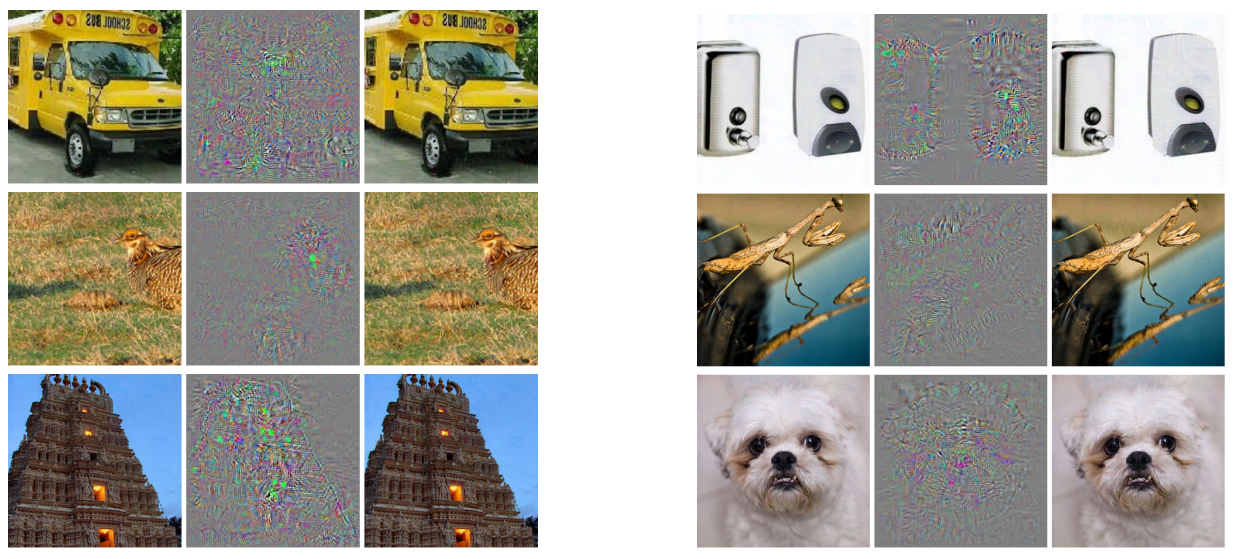
\includegraphics[width=0.85\textwidth]{./images/adversarial_examples.png}
%     % \caption{نمونه‌های دشمنانه\protect\LTRfootnote{\lr{Adversarial Examples}} تولید شده برای شبکه \lr{AlexNet} \cite{krizhevsky2012imagenet}. (چپ) نمونه‌ای که به‌درستی دسته‌بندی شده است، (وسط) تفاوت میان تصویر صحیح و تصویری که به‌اشتباه دسته‌بندی شده با بزرگ‌نمایی ۱۰ برابر (مقادیر با ۱۲۸ جمع و برش داده شده‌اند)، (راست) نمونه‌ دشمنانه. تمام تصاویر در ستون راست به‌عنوان «شترمرغ» پیش‌بینی شده‌اند. \cite{szegedy2014intriguing}}
%     \caption{نمونه‌های دشمنانه تولید شده برای شبکه \lr{AlexNet} \cite{krizhevsky2012imagenet}. (چپ) نمونه‌ای که به‌درستی دسته‌بندی شده است، (وسط) تفاوت میان تصویر صحیح و تصویری که به‌اشتباه دسته‌بندی شده با بزرگ‌نمایی ۱۰ برابر (مقادیر با ۱۲۸ جمع و برش داده شده‌اند)، (راست) نمونه‌ دشمنانه. تمام تصاویر در ستون راست به‌عنوان «شترمرغ» پیش‌بینی شده‌اند. \cite{szegedy2014intriguing}}
%     \label{fig:adversarial_examples}
%   \end{center}
% \end{figure}

\begin{figure}[h]
  \begin{center}
    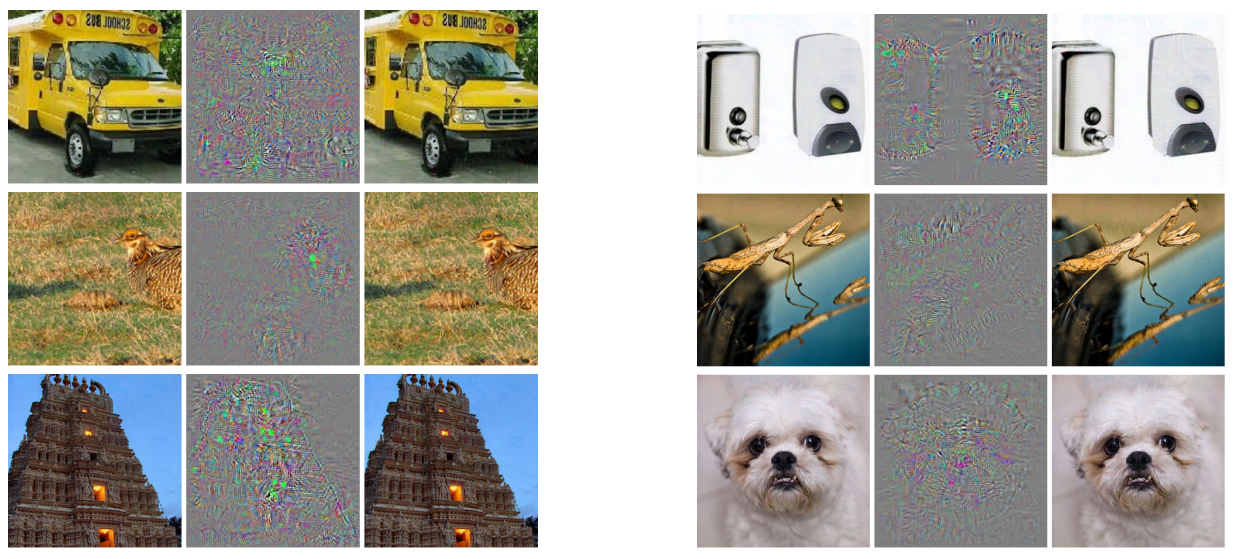
\includegraphics[width=0.85\textwidth]{./images/adversarial_examples.png}
    \stepcounter{endnote}%
    \edef\enoteA{\theendnote}%
    \endnotetext{\lr{Adversarial Examples}}%
    \caption{نمونه‌های دشمنانه\hbox{$^{\enoteA}$} تولید شده برای شبکه \lr{AlexNet} \cite{krizhevsky2012imagenet}. (چپ) نمونه‌ای که به‌درستی دسته‌بندی شده است، (وسط) تفاوت میان تصویر صحیح و تصویری که به‌اشتباه دسته‌بندی شده با بزرگ‌نمایی ۱۰ برابر (مقادیر با ۱۲۸ جمع و برش داده شده‌اند)، (راست) نمونه‌ دشمنانه. تمام تصاویر در ستون راست به‌عنوان «شترمرغ» پیش‌بینی شده‌اند. \cite{szegedy2014intriguing}}
    \label{fig:adversarial_examples}
  \end{center}
\end{figure}


\subsection{تعریف مسئله}

حمله‌ دشمنانه به افزودن آشفتگی‌ای کوچک و معمولاً نامحسوس به ورودی گفته می‌شود
که می‌تواند پیش‌بینی مدل را با اطمینان بالا نادرست کند.
\textbf{آموزش دشمنانه} یکی از مؤثرترین راهکارها برای مقاوم‌سازی مدل در برابر چنین حملاتی است
که در آن مدل به‌جای داده‌های تمیز، روی نمونه‌های دستکاری‌شده‌ دشمنانه آموزش می‌بیند\cite{madry2018towards}.
اما نسخه‌های چندمرحله‌ای آموزش دشمنانه به‌دلیل نیاز به چندین گام محاسبه‌ گرادیان در هر تکرار آموزش،
هزینه‌ محاسباتی بالایی دارند که مقیاس‌پذیری آن‌ها را محدود می‌کند.

برای کاهش این هزینه، \textbf{آموزش دشمنانه سریع} مبتنی بر حملات تک‌مرحله‌ای معرفی شد\cite{wong2020fast}.
این روش‌ها به‌مراتب کارآمدترند، اما چالش تازه‌ای به‌نام \textbf{بیش‌برازش فاجعه‌بار} را پدید می‌آورند:
پس از چند دوره‌ آموزشی\LTRfootnote{\lr{Training Epoch}}، درستی مقاوم\LTRfootnote{\lr{Robust Accuracy}} مدل در برابر حملات چندمرحله‌ای به‌طور ناگهانی به نزدیک صفر سقوط می‌کند،
در حالی‌که درستی\LTRfootnote{\lr{Accuracy}} آن در برابر همان حمله‌ تک‌مرحله‌ای که در آموزش به‌کار رفته است، حتی افزایش می‌یابد.

% Also can use the Figure 4 in the "FAST IS BETTER THAN FREE:REVISITING ADVERSARIAL TRAINING" paper.
\begin{figure}[h]
  \begin{center}
    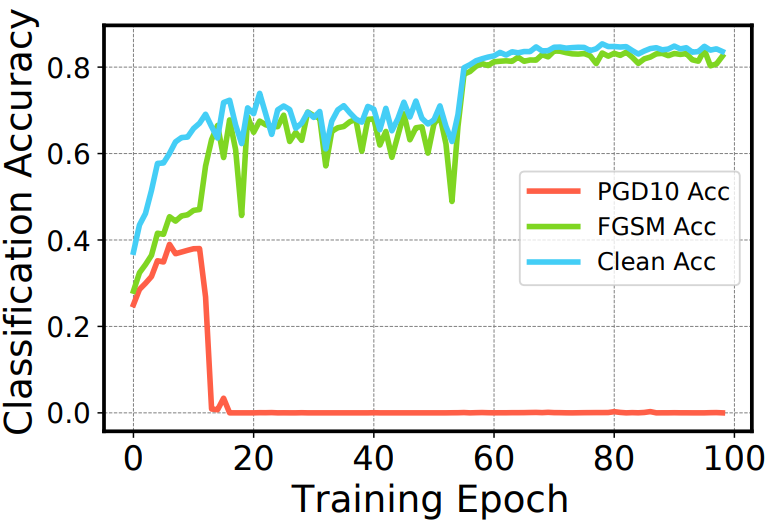
\includegraphics[width=0.45\textwidth]{./images/catastrophic_overfitting.png}
    \caption{پدیده‌ی بیش‌برازش فاجعه‌بار در آموزش دشمنانه‌ سریع. نمودار درستی دسته‌بندی را برای داده‌های تمیز، حمله‌ تک‌مرحله‌ای \lr{FGSM}، و حمله‌ چندمرحله‌ای \lr{PGD-10} در ۱۰۰ دوره‌ آموزشی برای مدل \lr{ResNet18} روی مجموعه‌داده‌ی \lr{CIFAR-10} نشان می‌دهد. همان‌گونه که مشاهده می‌شود، درستی در برابر حمله‌ \lr{FGSM} به‌سرعت افزایش می‌یابد، اما درستی مقاوم در برابر حمله‌ قوی‌تر \lr{PGD-10} به‌طور ناگهانی به نزدیک صفر سقوط می‌کند. \cite{wang2024preventing}}
    \label{fig:catastrophic_overfitting}
  \end{center}
\end{figure}

همان‌گونه که در شکل \ref{fig:catastrophic_overfitting} نشان داده شده است،
این پدیده بسیار نگران‌کننده است زیرا مدل در ظاهر عملکرد خوبی از خود نشان می‌دهد
(درستی بالا در برابر حمله‌ \lr{FGSM})، اما در عمل در برابر حملات قوی‌تر کاملاً شکننده است.
مسئله‌ اصلی مورد توجه در این سمینار، شناخت سازوکار بیش‌برازش فاجعه‌بار
و به‌ویژه \textbf{پیش‌بینی} زمان وقوع آن به‌جای صرفاً واکنش پس از رخ‌دادن آن است.

\subsection{اهمیت موضوع}

اهمیت پرداختن به این مسئله از چند جنبه قابل بررسی است:

\begin{itemize}
\item قوام دشمنانه در کاربردهای حساس به امنیت مانند خودروهای خودران، تشخیص پزشکی و سیستم‌های مالی نقشی حیاتی دارد و شکست مدل در برابر حملات می‌تواند پیامدهای جدی به همراه داشته باشد.
\item آموزش دشمنانه‌ چندمرحله‌ای هرچند مؤثر است، هزینه‌ محاسباتی بالایی دارد که مقیاس‌پذیری آن را روی مجموعه‌داده‌ها و معماری‌های بزرگ محدود می‌کند.
\item آموزش دشمنانه سریع راه‌حلی کارآمد است، اما تا زمانی که مسئله‌ بیش‌برازش فاجعه‌بار حل نشده باشد، قابل اعتماد نخواهد بود.
\item بسیاری از روش‌های موجود برای جلوگیری از بیش‌برازش فاجعه‌بار به تنظیم پرهزینه‌ ابرپارامترها یا محاسبات اضافی نیاز دارند که هدف اولیه‌ی آموزش دشمنانه سریع، یعنی قوام با کمترین هزینه، را تضعیف می‌کند.
\end{itemize}

از این رو، پیش‌بینی به‌موقع و کم‌هزینه‌ بیش‌برازش فاجعه‌بار می‌تواند
قابلیت اطمینان آموزش دشمنانه سریع را بدون افزایش هزینه‌ محاسباتی ارتقا دهد.

\subsection{اهداف و ساختار سمینار}\label{بخش:اهداف}

هدف این سمینار، مرور مفاهیم پایه و کارهای پیشین در زمینه‌ بیش‌برازش فاجعه‌بار در آموزش دشمنانه سریع،
و معرفی مختصر یک رویکرد برای پیش‌بینی و کنترل آن است.
ساختار ادامه‌ نوشتار به این صورت است:
در فصل~\ref{بخش:مفاهیم} مفاهیم اولیه شامل حملات دشمنانه، آموزش دشمنانه، آموزش دشمنانه سریع و بیش‌برازش فاجعه‌بار معرفی می‌شوند.
در فصل~\ref{بخش:کارهای‌پیشین} کارهای پیشین مرتبط دسته‌بندی و بررسی می‌شوند.
در فصل~\ref{بخش:روش} به‌اختصار به ایده‌ روش مورد بررسی پرداخته می‌شود
و در فصل~\ref{بخش:نتیجه} جمع‌بندی ارائه می‌گردد.


\section{مفاهیم اولیه}\label{بخش:مفاهیم}

در این فصل، مفاهیم بنیادینی که در ادامه‌ سمینار به آن‌ها نیاز است معرفی می‌شوند.
این مفاهیم شامل تعریف دقیق حملات دشمنانه، صورت‌بندی آموزش دشمنانه،
گذار به آموزش دشمنانه سریع، و سرانجام معرفی پدیده‌ بیش‌برازش فاجعه‌بار است.

\subsection{حملات دشمنانه و قوام}

% \شروع{تعریف}[نمونه دشمنانه] %% need to be revised (% -------------------- Environments -------------------- \newtheorem{تعریف}{تعریف}[chapter])
فرض کنید $f_{\theta}$ یک دسته‌بند\LTRfootnote{\lr{Classifier}} با پارامترهای $\theta$ و $(x, y)$ یک نمونه‌ ورودی به‌همراه برچسب درست آن باشد.
\textbf{نمونه دشمنانه} نمونه‌ای مانند $x + \delta$ است که در آن آشفتگی $\delta$ در یک کره‌ی $\ell_{\infty}$ به شعاع $\epsilon$ محدود شده است،
یعنی $\|\delta\|_{\infty} \le \epsilon$، و به‌گونه‌ای انتخاب می‌شود که مدل آن را نادرست دسته‌بندی کند.
% \پایان{تعریف}

ساده‌ترین و پرکاربردترین حمله‌ تک‌مرحله‌ای، روش علامت گرادیان سریع است
که آشفتگی را در جهت علامت گرادیان تابع اتلاف نسبت به ورودی می‌سازد \cite{goodfellow2015explaining}:

\begin{equation}
\delta = \epsilon \cdot \mathrm{sign}\!\left( \nabla_{x} \mathcal{L}(f_{\theta}(x), y) \right).
\end{equation}

در این رابطه، $\epsilon$ شعاع آشفتگی مجاز (معمولاً مقدار کوچکی مانند $\frac{8}{255}$ برای تصاویر) است،
$\mathcal{L}$ تابع اتلاف (معمولاً اتلاف بی‌نظمی متقاطع\LTRfootnote{\lr{Cross-Entropy Loss}}) است،
و $\mathrm{sign}(\cdot)$ تابع علامت است که خروجی آن برای ورودی‌های مثبت $+1$ و برای ورودی‌های منفی $-1$ خواهد بود.
بنابراین آشفتگی $\delta$ در هر بُعد، گامی به اندازه‌ $\epsilon$ در جهت افزایش اتلاف برمی‌دارد.

در مقابل، حمله‌ قوی‌تر و چندمرحله‌ای فرود گرادیان افکنش‌شده،
با تکرار گام‌های کوچک و افکنش آشفتگی روی کره‌ی مجاز به دست می‌آید~\cite{madry2018towards}:

\begin{equation}
x^{t+1} = \Pi_{\|x'-x\|_{\infty}\le\epsilon}\!\left( x^{t} + \alpha \cdot \mathrm{sign}\!\left( \nabla_{x} \mathcal{L}(f_{\theta}(x^{t}), y) \right) \right),
\end{equation}

که در آن $x^{t}$ نمونه‌ دشمنانه در گام $t$اُم است (با شروع از $x^{0} = x$)،
$x^{t+1}$ نمونه‌ دشمنانه‌ به‌روزرسانی‌شده در گام بعدی است،
$\alpha$ اندازه‌ گام در هر تکرار (معمولاً کوچک‌تر از $\epsilon$، مانند $\frac{2}{255}$) است،
و $\Pi$ عملگر افکنش\LTRfootnote{\lr{Projection Operator}} روی ناحیه‌ی مجاز $\|x'-x\|_{\infty}\le\epsilon$ است
که تضمین می‌کند آشفتگی نهایی از شعاع $\epsilon$ فراتر نرود.
این فرایند معمولاً برای چندین گام (برای مثال ۱۰ یا ۲۰ گام) تکرار می‌شود
که با نماد \lr{PGD-10} یا \lr{PGD-20} نشان داده می‌شود.
به درستی مدل در برابر چنین حملاتی، \textbf{درستی مقاوم}\LTRfootnote{\lr{Robust Accuracy}} گفته می‌شود.

\subsection{آموزش دشمنانه}

آموزش دشمنانه را می‌توان به‌صورت یک مسئله‌ بهینه‌سازی\LTRfootnote{\lr{Optimization}} کمینه‌بیشینه\LTRfootnote{\lr{Min-Max}} صورت‌بندی کرد،
که در آن بیشینه‌سازی درونی به‌دنبال یافتن آشفتگی‌ای است که تابع اتلاف را بیشینه کند،
و کمینه‌سازی بیرونی پارامترهای مدل را برای کاهش این اتلاف به‌روزرسانی می‌کند~\cite{madry2018towards}:

\begin{equation}
\min_{\theta} \; \mathbb{E}_{(x,y)\sim\mathcal{D}} \left[ \max_{\|\delta\|_{\infty}\le\epsilon} \mathcal{L}(f_{\theta}(x+\delta), y) \right].
\end{equation}

در این فرمول، $\min_{\theta}$ کمینه‌سازی بیرونی را نشان می‌دهد که پارامترهای مدل $\theta$ را برای کاهش اتلاف بهینه می‌کند،
$\mathbb{E}_{(x,y)\sim\mathcal{D}}$ امید ریاضی روی توزیع داده‌ی $\mathcal{D}$ است
(یعنی میانگین روی تمام نمونه‌های مجموعه‌داده‌ آموزشی)،
و $\max_{\|\delta\|_{\infty}\le\epsilon}$ بیشینه‌سازی درونی است
که به‌دنبال یافتن بدترین آشفتگی $\delta$ در همسایگی $\ell_{\infty}$ به شعاع $\epsilon$ است.
تابع اتلاف $\mathcal{L}$ نیز معمولاً اتلاف بی‌نظمی متقاطع است.
بنابراین، هدف نهایی یافتن پارامترهایی است که مدل را در برابر بدترین حمله‌ ممکن در همسایگی هر نمونه مقاوم سازد.

در روش استاندارد چندمرحله‌ای، بیشینه‌سازی درونی با حمله‌ فرود گرادیان افکنش‌شده حل می‌شود.
این رویکرد مؤثر است، اما به‌دلیل نیاز به چندین گام محاسبه‌ گرادیان (مانند ۱۰ گام در \lr{PGD-10}) در هر تکرار آموزش،
هزینه‌ محاسباتی آموزش را برای مدل‌ها و مجموعه‌داده‌های بزرگ به‌شدت افزایش می‌دهد.
برای مثال، آموزش دشمنانه با \lr{PGD-10} روی یک مدل متوسط می‌تواند تا ۱۰ برابر آموزش استاندارد زمان ببرد.

\subsection{آموزش دشمنانه سریع}

برای کاهش این هزینه، خانواده‌ای از روش‌ها با عنوان آموزش دشمنانه سریع معرفی شدند
که بیشینه‌سازی درونی را تنها با یک گام (مانند حمله‌ علامت گرادیان سریع) تقریب می‌زنند~\cite{wong2020fast}.
این روش‌ها هزینه‌ آموزش را به کسری از حالت چندمرحله‌ای کاهش می‌دهند.
یکی از مشاهدات کلیدی آن بوده که افزودن یک \textbf{شروع تصادفی}\LTRfootnote{\lr{Random Start}} به آشفتگی اولیه،
می‌تواند پایداری آموزش را بهبود بخشد.
با این حال، آموزش تک‌مرحله‌ای مستعد یک حالت شکست مشخص است که در ادامه معرفی می‌شود.

\subsection{بیش‌برازش فاجعه‌بار}

% \begin{تعریف}[بیش‌برازش فاجعه‌بار]  %% need to be revised (% -------------------- Environments -------------------- \newtheorem{تعریف}{تعریف}[chapter])
\textbf{بیش‌برازش فاجعه‌بار} پدیده‌ای است که عمدتاً در آموزش دشمنانه‌ تک‌مرحله‌ای رخ می‌دهد
و در آن، درستی مقاوم مدل در برابر حملات چندمرحله‌ای مانند فرود گرادیان افکنش‌شده،
تنها در عرض چند دوره آموزشی به‌طور ناگهانی به نزدیک صفر سقوط می‌کند،
در حالی‌که درستی در برابر حمله‌ تک‌مرحله‌ای به‌سرعت افزایش می‌یابد.
% \end{تعریف}

ویژگی قابل‌توجه بیش‌برازش فاجعه‌بار آن است که درستی تمیز مدل را کاهش نمی‌دهد
و گاه درستی در برابر حمله‌ تک‌مرحله‌ای حتی از درستی تمیز نیز فراتر می‌رود.
این موضوع نشان می‌دهد که مدل به‌جای کسب قوام واقعی،
صرفاً به حمله‌ خاص به‌کاررفته در آموزش بیش‌برازش کرده است و در برابر حملات قوی‌تر شکننده می‌شود.

یک دیدگاه پذیرفته‌شده، بیش‌برازش فاجعه‌بار را به تغییر در هندسه‌ی
\textbf{چشم‌انداز تابع اتلاف}\LTRfootnote{\lr{Loss Function Landscape}} نسبت می‌دهد؛
به‌گونه‌ای که در آستانه‌ وقوع آن، سطح اتلاف به‌شدت غیرخطی و مخدوش می‌شود~\cite{kim2021understanding,kang2021understanding}.
این غیرخطی‌شدن باعث می‌شود آشفتگی تک‌مرحله‌ای دیگر نتواند بیشینه‌ محلی واقعی اتلاف را هدف بگیرد
و در نتیجه نمونه‌های دشمنانه‌ نامناسبی تولید شوند.

\begin{figure}[t]
  \begin{center}
    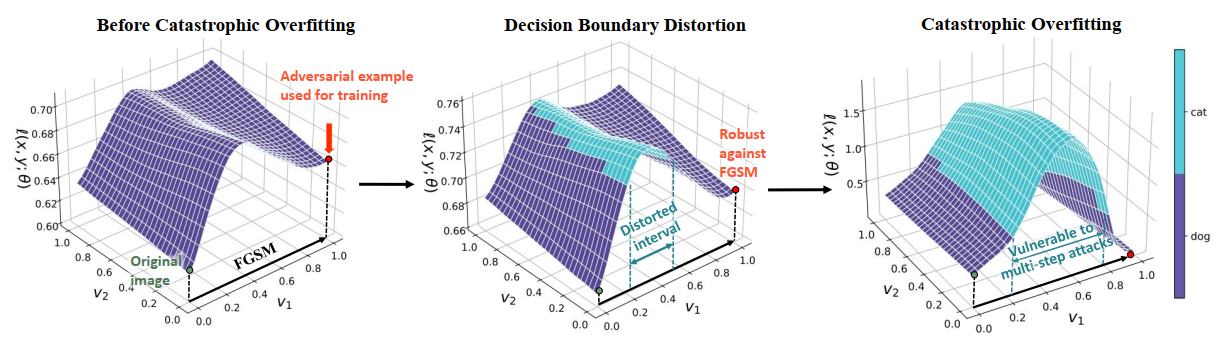
\includegraphics[width=0.95\textwidth]{./images/loss_landscape_distortion.png}
    \caption{فرایند اعوجاج مرز تصمیم‌گیری در اثر بیش‌برازش فاجعه‌بار. (چپ) سطح اتلاف پیش از وقوع بیش‌برازش فاجعه‌بار، به‌همراه جهت دشمنانه‌ \lr{FGSM} با بردار $v_1$ و یک جهت تصادفی $v_2$. نقطه‌ قرمز، نمونه‌ دشمنانه‌ $x+v_1$ تولیدشده از تصویر اصلی $x$ با برچسب «سگ» را نشان می‌دهد. (وسط) تغییر سطح اتلاف پس از یادگیری نمونه‌ دشمنانه‌ $x+v_1$. بردار $v_1$ همان بردار شکل سمت چپ است. ناحیه‌ی اعوجاج‌یافته برای نخستین بار ظاهر می‌شود. (راست) با ادامه‌ی آموزش، مرز تصمیم‌گیری مخدوش به‌طور کنترل‌نشده‌ای رشد می‌کند، به‌گونه‌ای که قوام در برابر حملات دشمنانه‌ چندمرحله‌ای کاهش می‌یابد. \cite{kim2021understanding}}
    \label{fig:loss_landscape_distortion}
  \end{center}
\end{figure}

همان‌گونه که در شکل \ref{fig:loss_landscape_distortion} نشان داده شده است،
پیش از وقوع بیش‌برازش فاجعه‌بار (تصویر سمت چپ)، سطح اتلاف نسبتاً هموار است
و جهت حمله‌ \lr{FGSM} (بردار $v_1$) به‌درستی به سمت ناحیه‌ای با اتلاف بالا اشاره می‌کند.
اما با ادامه‌ی آموزش (تصویر وسط)، سطح اتلاف در اطراف نمونه‌ دشمنانه شروع به اعوجاج می‌کند
و نواحی غیرخطی و معوج\LTRfootnote{\lr{Distorted Intervals}} پدیدار می‌شوند.
در نهایت (تصویر راست)، این اعوجاج به‌طور کنترل‌نشده‌ای گسترش می‌یابد
و مرز تصمیم‌گیری را چنان مخدوش می‌کند که حمله‌ تک‌مرحله‌ای دیگر نمی‌تواند
بیشینه‌ واقعی اتلاف را هدف قرار دهد و قوام در برابر حملات چندمرحله‌ای از بین می‌رود.

\subsection{انحنا و دیدگاه مرتبه دوم}

ارتباط نزدیکی میان \textbf{انحنای}\LTRfootnote{\lr{Curvature}} چشم‌انداز تابع اتلاف و قوام مدل وجود دارد.
هرچه سطح اتلاف در اطراف یک نمونه هموارتر (کم‌انحناتر) باشد،
حمله‌ تک‌مرحله‌ای تقریب بهتری از بیشینه‌ واقعی اتلاف ارائه می‌دهد.
از همین رو، اطلاعات مرتبه دوم (مانند ماتریس هسی\LTRfootnote{\lr{Hessian}}) می‌توانند در تحلیل و کنترل بیش‌برازش فاجعه‌بار سودمند باشند؛
هرچند محاسبه‌ مستقیم آن‌ها برای مسائل بزرگ‌مقیاس پرهزینه است.
این مشاهده انگیزه‌ای برای روش‌هایی است که می‌کوشند اطلاعات انحنا را به‌صورت غیرمستقیم و کم‌هزینه تقریب بزنند.

% \subsection{معیارهای ارزیابی\LTRfootnote{\lr{Evaluation}}}
\subsection[معیارهای ارزیابی]{معیارهای ارزیابی\LTRfootnote{\lr{Evaluation Metrics}}}

برای ارزیابی قوام مدل‌ها معمولاً از درستی در برابر حملات گوناگون استفاده می‌شود.
درستی در برابر حمله‌ تک‌مرحله‌ای به‌تنهایی می‌تواند گمراه‌کننده باشد،
زیرا در حضور بیش‌برازش فاجعه‌بار بالا می‌ماند.
بنابراین ارزیابی قابل‌اعتماد معمولاً با حملات چندمرحله‌ای و به‌ویژه با
مجموعه‌حمله‌ استاندارد و بدون‌پارامتر \lr{AutoAttack} انجام می‌شود~\cite{croce2020reliable}.
افزون بر این، \textbf{بده‌بستان درستی مقاوم-تمیز}\LTRfootnote{\lr{Robustness-Accuracy Trade-off}}
یکی از معیارهای مهم در مقایسه‌ی روش‌هاست~\cite{tsipras2019robustness}.

\section{کارهای پیشین}\label{بخش:کارهای‌پیشین}

پژوهش‌های فراوانی به تبیین و رفع بیش‌برازش فاجعه‌بار پرداخته‌اند.
در این فصل، مهم‌ترین آن‌ها بر اساس راهبرد اصلی مقابله با این پدیده دسته‌بندی و بررسی می‌شوند.

\subsection{روش‌های مبتنی بر تصادفی‌سازی}

این دسته از روش‌ها با تزریق تصادفی‌بودن به فرایند تولید نمونه‌ دشمنانه می‌کوشند از بیش‌برازش مضر جلوگیری کنند.
نشان داده شده است که افزودن یک شروع تصادفی به آموزش مبتنی بر علامت گرادیان سریع
می‌تواند تا حد زیادی از بیش‌برازش فاجعه‌بار جلوگیری کند~\cite{wong2020fast}.
این ایده بعدها با افزایش دامنه‌ نویز تصادفی و حذف گام برش\LTRfootnote{\lr{Clipping}} گسترش یافت
و روشی موسوم به \lr{N-FGSM} ارائه شد که هم قوام و هم درستی بهتری به دست می‌دهد~\cite{dejorge2022make}.

\begin{figure}[t]
  \begin{center}
    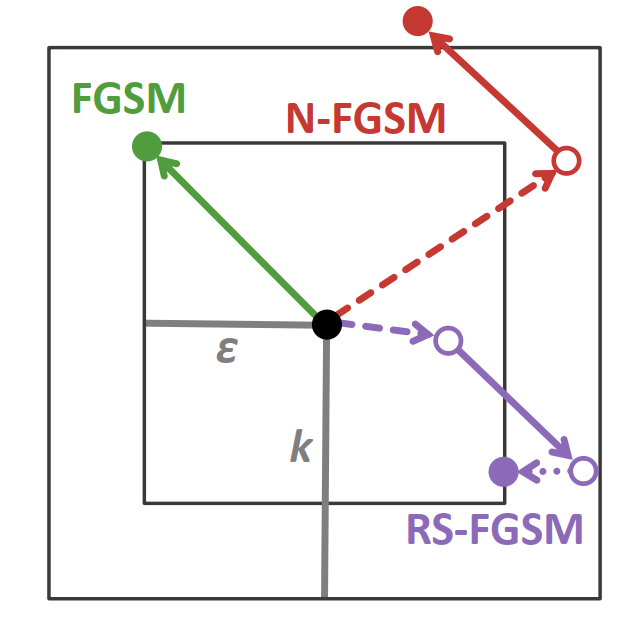
\includegraphics[width=0.35\textwidth]{./images/nfgsm_comparison.png}
    \caption{مقایسه‌ی تصویری حملات \lr{FGSM} \cite{goodfellow2015explaining}، \lr{RS-FGSM} \cite{wong2020fast} و \lr{N-FGSM} \cite{dejorge2022make}. در روش \lr{FGSM}، آشفتگی مستقیماً در جهت علامت گرادیان و بدون تصادفی‌سازی اعمال می‌شود. در روش \lr{RS-FGSM}، نویز تصادفی در یک کره‌ی $\ell_1$ به شعاع $\epsilon$ به نمونه اضافه و سپس برش داده می‌شود. اما در روش \lr{N-FGSM}، نویز از یک کره‌ی $\ell_1$ با شعاع دلخواه $k$ (معمولاً بزرگ‌تر از $\epsilon$) نمونه‌برداری می‌شود و گام برش نیز حذف می‌گردد، که منجر به تنوع بیشتر آشفتگی و قوام بهتر می‌شود.}
    \label{fig:nfgsm_comparison}
  \end{center}
\end{figure}

همان‌گونه که در شکل \ref{fig:nfgsm_comparison} مشاهده می‌شود،
تفاوت اصلی \lr{N-FGSM} با نسخه‌های پیشین در دو جنبه است:
نخست، استفاده از نویز تصادفی با دامنه‌ بزرگ‌تر (شعاع $k$ به‌جای $\epsilon$) که تنوع آشفتگی را افزایش می‌دهد،
و دوم، حذف گام برش که به آشفتگی اجازه می‌دهد آزادانه‌تر در فضای ورودی جستجو کند.
این دو تغییر ساده اما مؤثر، باعث می‌شوند \lr{N-FGSM} بتواند بدون گرفتار شدن در دام بیش‌برازش فاجعه‌بار،
قوام بهتری نسبت به روش‌های پیشین کسب کند.

\subsection{روش‌های مبتنی بر منظم‌سازی}

روش‌های مبتنی بر منظم‌سازی\LTRfootnote{\lr{Regularization}} با افزودن جمله‌ای محدودکننده به تابع هدف،
رفتار مدل را به‌گونه‌ای مقید می‌کنند که از بیش‌برازش فاجعه‌بار جلوگیری شود.
یکی از روش‌های شناخته‌شده، بیشینه‌سازی \textbf{هم‌راستایی گرادیان}\LTRfootnote{\lr{Gradient Alignment}}
میان نمونه‌ تمیز و نمونه‌ آشفته\LTRfootnote{\lr{Perturbed}} در مجموعه‌ی آشفتگی است (روش \lr{GradAlign})~\cite{andriushchenko2020understanding}.
برخی روش‌ها با استفاده از منظم‌سازی مبتنی بر نُرم، هموارسازی تابع را در همسایگی نمونه‌ها تقویت می‌کنند~\cite{sriramanan2021towards}.
دسته‌ای دیگر، \textbf{نمونه‌های دشمنانه‌ ناهنجار}\LTRfootnote{\lr{Abnormal Adversarial Examples}} را به‌عنوان منشأ بیش‌برازش فاجعه‌بار شناسایی کرده
و آن‌ها را با منظم‌سازی مهار می‌کنند (روش \lr{AAER})~\cite{lin2023eliminating}.
همچنین برخی پژوهش‌ها با تشویق \textbf{خطی‌بودن محلی}\LTRfootnote{\lr{Local Linearity}} سطح اتلاف،
به‌صورت کارآمد از این پدیده جلوگیری می‌کنند (روش \lr{ELLE})~\cite{rocamora2024efficient}.

\subsection{روش‌های مبتنی بر اندازه‌ گام تطبیقی}

این روش‌ها اندازه‌ گام حمله را بر اساس دینامیک آموزش تنظیم می‌کنند.
برخی از یادگیری تقویتی برای تعیین اندازه‌ گام بهره گرفته‌اند~\cite{nie2021adaptive}،
برخی دیگر اندازه‌ گام را با استفاده از نُرم گرادیان تطبیق داده‌اند~\cite{huang2023fast}،
و در پژوهشی دیگر اندازه‌ گام برای هر نمونه بر پایه‌ی شباهت میان نویز ورودی و جهت گرادیان تعیین شده است~\cite{zhao2025avoiding}.
ایده‌ مشترک این دسته آن است که با پرهیز از درون‌یابی در نواحی به‌شدت غیرخطی،
می‌توان از تولید نمونه‌های دشمنانه‌ نامناسب و در نتیجه از بیش‌برازش فاجعه‌بار جلوگیری کرد.

\subsection{سایر رویکردها}

برخی روش‌ها از منظرهای دیگری به مسئله می‌نگرند.
به‌عنوان نمونه، حذف به‌روزرسانی‌هایی با اندازه‌ گرادیان ناچیز برای پایدارسازی آموزش پیشنهاد شده است~\cite{golgooni2023zerograd}.
همچنین روش آموزش دشمنانه‌ رایگان\LTRfootnote{\lr{Free Adversarial Training}}
با استفاده‌ هم‌زمان از گرادیان تولید نمونه‌ دشمنانه برای به‌روزرسانی وزن‌ها،
سربار محاسباتی حمله را حذف می‌کند~\cite{shafahi2019adversarial}.

\subsection{بهینه‌سازی مرتبه دوم و قوام}

دسته‌ای از پژوهش‌ها با الهام از ارتباط میان انحنا و قوام،
از منظم‌سازی انحنا برای آموزش مدل‌های مقاوم استفاده کرده‌اند~\cite{moosavi2019robustness}.
این رویکردها نشان می‌دهند که کنترل اطلاعات مرتبه دوم سطح اتلاف می‌تواند در بهبود قوام مؤثر باشد،
هرچند تاکنون کمتر در چارچوب آموزش دشمنانه سریع و کم‌هزینه به‌کار رفته‌اند.

\subsection{معیارهای پیش‌بینی بیش‌برازش فاجعه‌بار}

تاکنون معیار مشخصی که صرفاً برای پیش‌بینی کم‌هزینه‌ بیش‌برازش فاجعه‌بار طراحی شده باشد ارائه نشده است؛
با این حال چند سنجه می‌توانند به‌صورت غیرمستقیم نشانه‌ای زودهنگام از وقوع آن باشند،
مانند هم‌راستایی گرادیان~\cite{andriushchenko2020understanding}،
نرخ نمونه‌های دشمنانه‌ ناهنجار~\cite{lin2023eliminating}
و معیارهای غیرخطی‌بودن سطح اتلاف~\cite{rocamora2024efficient}.

\textbf{هم‌راستایی گرادیان} که در کار آندریوشچنکو و همکاران \cite{andriushchenko2020understanding} معرفی شده است،
میزان خطی‌بودن موضعی تابع اتلاف را به‌کمک شباهت کسینوسی میان گرادیان نمونه‌ تمیز
و گرادیان نمونه‌ آشفته با نویز تصادفی $\eta$ اندازه‌گیری می‌کند:

\begin{equation}
\mathbb{E}_{(x,y)\sim\mathcal{D},\; \eta\sim\mathcal{U}([-\epsilon,\epsilon]^d)} \left[ \cos\!\big( \nabla_x \mathcal{L}(x, y; \theta),\; \nabla_x \mathcal{L}(x+\eta, y; \theta) \big) \right].
\end{equation}

در این رابطه، $\mathbb{E}$ امید ریاضی روی تمام نمونه‌های داده و نویز تصادفی است،
$\eta \sim \mathcal{U}([-\epsilon,\epsilon]^d)$ نویزی است که به‌طور یکنواخت از بازه‌ی $[-\epsilon,\epsilon]$ در هر بُعد نمونه‌برداری می‌شود،
و $\cos(\cdot,\cdot)$ شباهت کسینوسی میان دو بردار گرادیان را محاسبه می‌کند
که اگر دو بردار هم‌جهت باشند ۱ و اگر عمود باشند ۰ خواهد بود.
هرچه این مقدار به ۱ نزدیک‌تر باشد، سطح اتلاف در همسایگی $\epsilon$ خطی‌تر است
و حمله‌ \lr{FGSM} تقریب دقیق‌تری از بیشینه‌ واقعی اتلاف ارائه می‌دهد.
کاهش ناگهانی این معیار می‌تواند هشداری برای وقوع قریب‌الوقوع بیش‌برازش فاجعه‌بار باشد،
اما محاسبه‌ آن نیازمند یک پس‌انتشار اضافی برای گرادیان $\nabla_x \mathcal{L}(x+\eta, y; \theta)$ است.

\textbf{نمونه‌های دشمنانه‌ ناهنجار} نیز توسط لین و همکاران \cite{lin2023eliminating} به‌عنوان نشانه‌ای از اعوجاج دسته‌بند معرفی شده‌اند.
اگر $x+\eta$ نمونه‌ آغشته به نویز تصادفی و $\delta$ آشفتگی \lr{FGSM} محاسبه‌شده روی آن باشد،
نمونه‌ای ناهنجار (\lr{AAE}) خوانده می‌شود که در آن افزودن آشفتگی، برخلاف انتظار،
اتلاف را \textit{کاهش} دهد:

\begin{equation}
\mathcal{L}(x+\eta, y; \theta) > \mathcal{L}(x+\eta+\delta, y; \theta).
\end{equation}

در این نامساوی، $\mathcal{L}(x+\eta, y; \theta)$ اتلاف مدل روی نمونه‌ نویزدار پیش از اعمال آشفتگی،
$\delta = \mathrm{sign}(\nabla_{x+\eta} \mathcal{L}(x+\eta, y; \theta))$ آشفتگی \lr{FGSM} محاسبه‌شده روی همان نمونه،
و $\mathcal{L}(x+\eta+\delta, y; \theta)$ اتلاف پس از افزودن آشفتگی است.
در حالت عادی انتظار می‌رود افزودن آشفتگی دشمنانه اتلاف را \textit{افزایش} دهد،
اما در نمونه‌های ناهنجار این رابطه برعکس می‌شود که نشانه‌ای از غیرخطی‌شدن شدید سطح اتلاف است.
پیش از وقوع بیش‌برازش فاجعه‌بار، شمار اندکی \lr{AAE} در داده‌های آموزشی ظاهر می‌شوند
که نشان‌دهنده‌ی آغاز اعوجاج مرز تصمیم‌گیری است؛
اما ردیابی آن‌ها نیز مستلزم ارزیابی اتلاف روی هر دو نقطه‌ پیش و پس از اعمال آشفتگی است.

مشکل مشترک این سنجه‌ها آن است که اغلب به محاسبات اضافی مانند پس‌انتشار یا عبور رو‌به‌جلو بیشتر نیاز دارند
و در نتیجه هزینه‌ محاسباتی آموزش را افزایش می‌دهند؛
چالشی که انگیزه‌ی اصلی پژوهش حاضر برای یافتن معیاری دقیق اما کم‌هزینه است.

\subsection{محدودیت‌های روش‌های پیشین}

علی‌رغم پیشرفت‌های قابل توجه، روش‌های پیشین همچنان با چالش‌های مهمی روبرو هستند:

\begin{enumerate}

\item
\textbf{وابستگی به مجموعه‌داده و معماری}:
اکثر روش‌ها برای مجموعه‌داده‌های استاندارد مثل \lr{CIFAR-10} تنظیم شده‌اند
و عملکرد آن‌ها در مجموعه‌داده‌های دیگر یا معماری‌های متفاوت قابل اطمینان نیست.

\item
\textbf{نیاز به تنظیم ابرپارامتر}:
بسیاری از روش‌ها برای هر مجموعه‌داده یا معماری نیاز به جستجوی مستقل ابرپارامتر دارند،
که این امر هزینه‌ کلی را افزایش می‌دهد.

\item
\textbf{هزینه‌ محاسباتی اضافی}:
برخی رویکردها مانند \lr{GradAlign} و \lr{ELLE} برای پیشگیری از بیش‌برازش فاجعه‌بار، هزینه‌ محاسباتی قابل توجهی نسبت به روش‌های پایه اضافه می‌کنند.

\item
\textbf{نبود معیار پیش‌بینی کارآمد}:
تاکنون، هیچ معیاری که بتواند به‌طور کارآمد وقوع قریب‌الوقوع بیش‌برازش فاجعه‌بار را پیش‌بینی کند وجود نداشته است.
معیارهای موجود مانند \lr{GradAlign} اگرچه می‌توانند نشانه‌هایی از شروع بیش‌برازش فاجعه‌بار بدهند،
اما هزینه‌ محاسباتی بالایی دارند.

برای جمع‌بندی و مقایسه‌ روشن‌تر روش‌های مرورشده در این فصل،
جدول~\ref{tab:comparison_prior_works} راهبرد اصلی، ویژگی کلیدی، مزیت و محدودیت هر یک از روش‌های پیشین را
در کنار هم ارائه می‌دهد. همان‌گونه که از این جدول برمی‌آید، هرچند هر دسته از روش‌ها
توانسته است بیش‌برازش فاجعه‌بار را تا حدی مهار کند، اما هیچ‌یک به‌طور هم‌زمان
هر چهار چالش برشمرده‌شده در بالا 
(یعنی وابستگی به مجموعه‌داده و معماری، نیاز به تنظیم ابرپارامتر، هزینه‌ محاسباتی اضافی و نبود معیار پیش‌بینی کارآمد)
را برطرف نکرده است؛
شکافی که انگیزه‌ اصلی رویکرد ارائه‌شده در فصل بعد است.


{\small
\renewcommand{\arraystretch}{1.3} %%  tighter row spacin
\setlength{\tabcolsep}{8pt} %% cell padding
\begin{longtable}{|p{2.2cm}|p{2cm}|p{3.2cm}|p{3.2cm}|p{3.2cm}|} %%  column width 
\caption{مقایسه‌ روش‌های پیشین در پیشگیری و پیش‌بینی بیش‌برازش فاجعه‌بار.}
\label{tab:comparison_prior_works} \\
\hline
\textbf{روش} & \textbf{راهبرد} & \textbf{ویژگی کلیدی} & \textbf{مزیت} & \textbf{محدودیت} \\
\hline
\endfirsthead
\multicolumn{5}{c}{\small ادامه‌ی جدول~\ref{tab:comparison_prior_works}} \\
\hline
\textbf{روش} & \textbf{راهبرد} & \textbf{ویژگی کلیدی} & \textbf{مزیت} & \textbf{محدودیت} \\
\hline
\endhead
\hline
\endfoot

\lr{FGSM-RS}~\cite{wong2020fast} & تصادفی‌سازی & افزودن شروع تصادفی پیش از آشفتگی \lr{FGSM} & ساده و تقریباً بدون سربار محاسباتی & در مقیاس‌های بزرگ‌تر $\epsilon$ همچنان مستعد بیش‌برازش فاجعه‌بار است \\
\hline
\lr{N-FGSM}~\cite{dejorge2022make} & تصادفی‌سازی & نویز با دامنه‌ بزرگ‌تر از $\epsilon$ و حذف گام برش & قوام و درستی بهتر نسبت به \lr{FGSM-RS} & دامنه‌ نویز نیازمند تنظیم و وابسته به مجموعه‌داده \\
\hline
\lr{GradAlign}~\cite{andriushchenko2020understanding} & منظم‌سازی & بیشینه‌سازی هم‌راستایی گرادیان نمونه‌ تمیز و آشفته & پایه‌ نظری روشن؛ معیاری برای پیش‌بینی نیز فراهم می‌کند & نیازمند پس‌انتشار اضافی و هزینه‌ محاسباتی قابل توجه \\
\hline
\lr{NuAT}~\cite{sriramanan2021towards} & منظم‌سازی & هموارسازی تابع اتلاف با منظم‌سازی نُرم اتمی & بهبود پایداری آموزش & هزینه‌ محاسباتی و حافظه‌ اضافی \\
\hline
\lr{AAER}~\cite{lin2023eliminating} & منظم‌سازی & شناسایی و مهار نمونه‌های دشمنانه‌ ناهنجار & ریشه‌یابی مستقیم یکی از علل بیش‌برازش فاجعه‌بار & نیازمند ارزیابی اتلاف در چند نقطه؛ حساس به تنظیم آستانه \\
\hline
\lr{ELLE}~\cite{rocamora2024efficient} & منظم‌سازی & تشویق خطی‌بودن محلی سطح اتلاف & قوام بالا و اثربخشی در مجموعه‌داده‌های چالش‌برانگیز & سربار محاسباتی و حافظه‌ای بالاتر از روش‌های پایه \\
\hline
\lr{RL-based}~\cite{nie2021adaptive} & گام تطبیقی & تعیین اندازه‌ گام با یادگیری تقویتی & تطبیق پویا با دینامیک آموزش & پیچیدگی پیاده‌سازی و هزینه‌ آموزش عامل تقویتی \\
\hline
\lr{ATAS}~\cite{huang2023fast} & گام تطبیقی & تطبیق اندازه‌ گام بر اساس نُرم گرادیان & کارآمد و بدون نیاز به مؤلفه‌ یادگیری جداگانه & عملکرد وابسته به کیفیت تخمین نُرم گرادیان در هر نمونه \\
\hline
روش تشابه گرادیان~\cite{zhao2025avoiding} & گام تطبیقی & تعیین گام برای هر نمونه بر پایه‌ شباهت نویز و جهت گرادیان & توجه ویژه به سطح نمونه به‌جای کل دسته & نیازمند محاسبات اضافی به ازای هر نمونه \\
\hline
\lr{ZeroGrad}~\cite{golgooni2023zerograd} & سایر رویکردها & حذف به‌روزرسانی‌های با گرادیان ناچیز & پیاده‌سازی بسیار ساده و کم‌هزینه & اثربخشی محدودتر روی مجموعه‌داده‌های دشوارتر \\
\hline
\lr{Free AT}~\cite{shafahi2019adversarial} & سایر رویکردها & بازاستفاده از گرادیان حمله برای به‌روزرسانی وزن‌ها & حذف کامل سربار محاسباتی حمله‌ جداگانه & درستی تمیز و قوام معمولاً پایین‌تر از روش‌های تخصصی‌تر \\
\hline
منظم‌سازی انحنا~\cite{moosavi2019robustness} & مرتبه دوم & کنترل مستقیم انحنای سطح اتلاف & پیوند نظری قوی میان انحنا و قوام & کمتر در چارچوب آموزش دشمنانه‌ سریع و کم‌هزینه به‌کار رفته است \\
\hline

\end{longtable}
}


\end{enumerate}

\section{روش ارائه شده}\label{بخش:روش}

با تکیه بر مفاهیم و کارهای پیشین مرورشده، رویکرد مورد بررسی در این سمینار بر سه ایده‌ به‌هم‌پیوسته استوار است:
مشاهده‌ تجربی نقش ثابت‌بودن اندازه و جهت آشفتگی در پیدایش بیش‌برازش فاجعه‌بار،
طراحی یک سنجه‌ کم‌هزینه برای پیش‌بینی زودهنگام این پدیده،
و در نهایت تعیین پویای اندازه‌ گام حمله بر پایه‌ دیدگاه مرتبه دوم.
در ادامه، برای هر یک از دو ایده‌ نخست، آزمایشی تجربی نیز ارائه می‌شود.

\subsection{بیش‌برازش شعاع آشفتگی مجاز ($\epsilon$)}\label{بخش:شاهد‌اپسیلون}

برای بررسی این فرضیه که ثابت و نسبتاً بزرگ‌بودن اندازه‌ آشفتگی حمله (بدون تنوع در اندازه یا جهت آن)
می‌تواند زمینه‌ساز بیش‌برازش فاجعه‌بار باشد، آزمایشی روی مدل \lr{PreActResNet18} در مجموعه‌داده‌ \lr{CIFAR10} انجام شد که با آشفتگی ثابت
$\epsilon = \frac{8}{255}$ آموزش دیده و دچار بیش‌برازش فاجعه‌بار شده است.
درستی این مدل در برابر حمله‌ \lr{FGSM} و حمله‌ \lr{PGD-10} برای بازه‌ای از مقادیر قدرت حمله
(از $-\frac{16}{255}$ تا $+\frac{16}{255}$) اندازه‌گیری و در شکل \ref{fig:epsilon_overfitting} گزارش شده است.

\begin{figure}[h]
  \begin{center}
    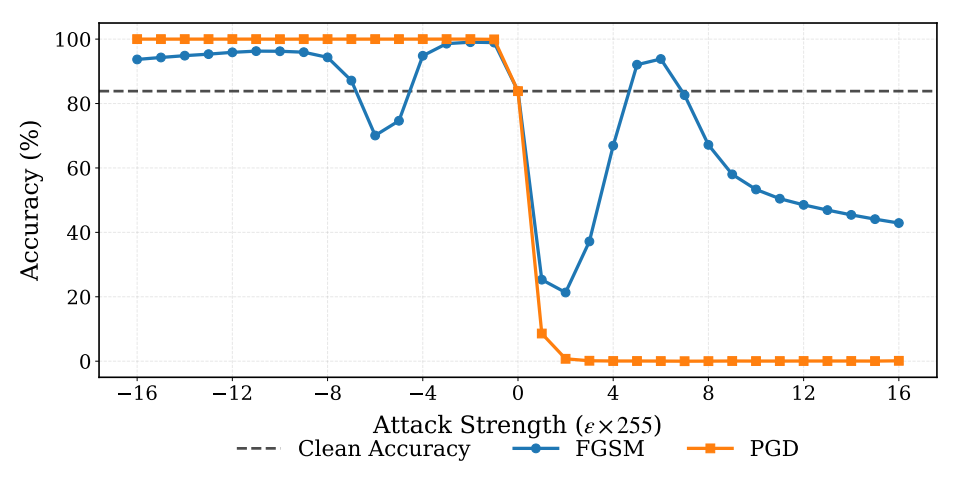
\includegraphics[width=0.6\textwidth]{./images/epsilon_overfitting_fgsm.png}
    \caption{درستی یک مدل دچار بیش‌برازش فاجعه‌بار (آموزش‌دیده با \lr{FGSM} و $\epsilon = \frac{8}{255}$) در برابر حمله‌ \lr{FGSM} و \lr{PGD-10}، به ازای مقادیر مختلف قدرت حمله. خط چین، درستی تمیز مدل را نشان می‌دهد.}
    \label{fig:epsilon_overfitting}
  \end{center}
\end{figure}

همان‌گونه که در شکل \ref{fig:epsilon_overfitting} دیده می‌شود، درستی \lr{FGSM} رفتاری بسیار نامنظم دارد:
برای برخی مقادیر $\epsilon$ (از جمله همان مقداری که در آموزش به‌کار رفته) به‌شدت بالا می‌ماند،
در حالی‌که برای مقادیر دیگر، حتی نزدیک به همان بازه، به‌طرز غیرمنتظره‌ای افت می‌کند.
این نوسان شدید نشان می‌دهد که سطح اتلاف، حتی در طول همان جهت آشفتگی‌ای که در آموزش استفاده شده،
به‌شدت غیرخطی و ناهموار شده است؛ به بیان دیگر، مدل به‌جای کسب قوام واقعی،
تنها به مقادیر مشخصی از اندازه‌ آشفتگی بیش‌برازش کرده است، پدیده‌ای که آن را
\textbf{بیش‌برازش اپسیلون}\LTRfootnote{\lr{Epsilon Overfitting}} می‌نامیم.
در مقابل، درستی در برابر \lr{PGD-10} در تقریباً تمام این بازه پایین و نزدیک صفر باقی می‌ماند،
که تأیید می‌کند نوسانات درستی \lr{FGSM} بازتابی از قوام واقعی مدل نیست،
بلکه صرفاً برازشی موضعی و شکننده به شکل خاصی از آشفتگی است.
این مشاهده، انگیزه‌ اصلی افزودن تنوع به توزیع اندازه و جهت آشفتگی حمله است.

\subsection{سنجه‌ پیش‌بینی: هم‌ترازی آشفتگی}\label{بخش:پرتالاین}

برای پیش‌بینی کم‌هزینه‌ بیش‌برازش فاجعه‌بار، پیش از افت محسوس درستی مقاوم،
سنجه‌ای مبتنی بر گرادیان تعریف می‌شود که آن را \textbf{هم‌ترازی آشفتگی} می‌نامیم.
این سنجه، شباهت کسینوسی میان دو گرادیان را اندازه می‌گیرد:
گرادیان اتلاف نسبت به نمونه‌ دارای شروع تصادفی و گرادیان اتلاف پس از برداشتن یک گام اضافی
در جهت حمله روی همان نمونه. در واقع:

\begin{equation}
\text{هم‌ترازی آشفتگی} = \cos\!\Big( \nabla_{x} \mathcal{L}\big(f_{\theta}(x'), y\big),\; \nabla_{x} \mathcal{L}\big(f_{\theta}(x'+\delta), y\big) \Big),
\end{equation}

که در آن $x' = x + \eta$ نمونه‌ دارای شروع تصادفی $\eta \sim \mathcal{U}([-\epsilon,\epsilon]^d)$ است
و $\delta = \alpha \cdot \mathrm{sign}\big(\nabla_x \mathcal{L}(f_\theta(x'), y)\big)$ گامی به اندازه‌ $\alpha$
در جهت حمله است.
اگر سطح اتلاف در همسایگی نمونه به‌طور محلی خطی باشد، گرادیان اتلاف در طول این دو نقطه‌ نزدیک به‌هم
تغییر چندانی نمی‌کند و در نتیجه هم‌ترازی آشفتگی به ۱ نزدیک می‌ماند.
اما در آستانه‌ بیش‌برازش فاجعه‌بار که سطح اتلاف به‌شدت غیرخطی می‌شود،
جهت گرادیان میان این دو نقطه به‌سرعت تغییر می‌کند و هم‌ترازی آشفتگی به سمت صفر میل می‌کند.
نکته‌ مهم آن است که هر دو گرادیان مورد نیاز این سنجه،
در روند معمول تولید نمونه‌ دشمنانه و به‌روزرسانی وزن‌ها در آموزش تک‌مرحله‌ای، از پیش محاسبه می‌شوند؛
بنابراین محاسبه‌ این سنجه عملاً سربار محاسباتی اضافه‌ای در بر ندارد.

\begin{figure}[h]
  \begin{center}
    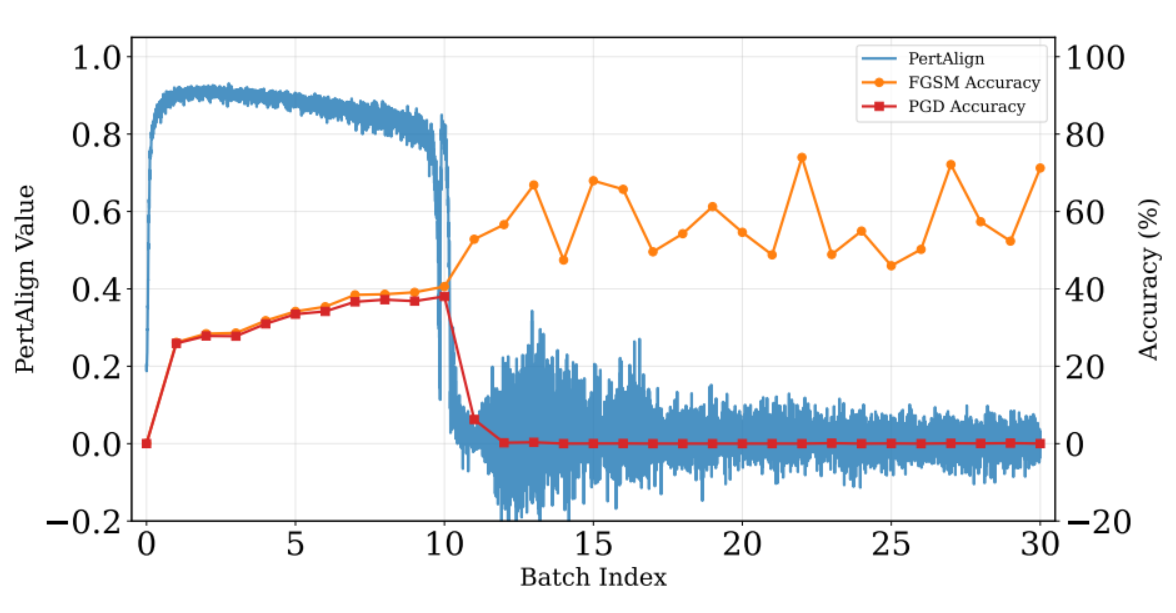
\includegraphics[width=0.6\textwidth]{./images/perturbation_alignment_PreActResNet_cifar10.png}
    \caption{روند درستی \lr{FGSM}، درستی \lr{PGD-10} و مقدار هم‌ترازی آشفتگی در طول آموزش دشمنانه‌ تک‌مرحله‌ای با معماری \lr{PreActResNet18} روی مجموعه‌داده‌ی \lr{CIFAR-10}. افت هم‌ترازی آشفتگی، پیش از واگرایی محسوس درستی \lr{FGSM} و \lr{PGD-10} (یعنی پیش از وقوع آشکار بیش‌برازش فاجعه‌بار) رخ می‌دهد.}
    \label{fig:pertalign_senet18}
  \end{center}
\end{figure}

همان‌گونه که در شکل \ref{fig:pertalign_senet18} مشاهده می‌شود، افت هم‌ترازی آشفتگی
زودتر از واگرایی درستی \lr{FGSM} و \lr{PGD-10} رخ می‌دهد و می‌تواند به‌عنوان هشداری زودهنگام
برای وقوع قریب‌الوقوع بیش‌برازش فاجعه‌بار عمل کند، بدون آنکه هزینه‌ محاسباتی محسوسی به آموزش تحمیل شود.

\subsection{ایده‌ کلی برای تنظیم پویای اندازه‌ گام}

با نگریستن به مسئله‌ بیشینه‌سازی اتلاف از دیدگاه بهینه‌سازی مرتبه دوم
و تقریب محلی سطح اتلاف با یک مدل درجه‌دوم،
می‌توان اندازه‌ گام بهینه‌ی حمله را به‌صورت پویا و متناسب با هندسه‌ محلی چشم‌انداز تابع اتلاف تعیین کرد؛
اندازه‌ گامی که با استفاده از همان اطلاعات به‌کاررفته در محاسبه‌ هم‌ترازی آشفتگی
و تقریباً بدون هزینه‌ اضافه به دست می‌آید.
ترکیب این سه ایده
(تنوع‌بخشی به توزیع آشفتگی برای جلوگیری از بیش برازش، پیش‌بینی کم‌هزینه با هم‌ترازی آشفتگی
و تعیین پویای اندازه‌ گام)
می‌تواند به روشی بینجامد که از وقوع بیش‌برازش فاجعه‌بار جلوگیری کند
و با یک مجموعه‌ ثابت از ابرپارامترها در دامنه‌ها و معماری‌های گوناگون قابل استفاده باشد.
جزئیات کامل چنین روشی، به‌همراه ارزیابی گسترده‌ آن روی مجموعه‌داده‌ها و معماری‌های متعدد،
موضوع پایان‌نامه‌ آینده خواهد بود.

\section{نتیجه‌گیری}\label{بخش:نتیجه}

در این سمینار، مسئله‌ بیش‌برازش فاجعه‌بار به‌عنوان اصلی‌ترین مانع در مسیر آموزش دشمنانه‌ سریع و کارآمد بررسی شد.
ابتدا مفاهیم پایه‌ای حملات دشمنانه، آموزش دشمنانه، آموزش دشمنانه سریع و خود پدیده‌ بیش‌برازش فاجعه‌بار
به‌همراه پیوند آن با هندسه و انحنای چشم‌انداز تابع اتلاف معرفی شدند.
سپس کارهای پیشین در قالب چند دسته‌ اصلی از جمله تصادفی‌سازی، منظم‌سازی، اندازه‌ گام تطبیقی،
سایر رویکردها و بهینه‌سازی مرتبه دوم مرور و نقاط ضعف آن‌ها،
به‌ویژه نیاز به تنظیم پرهزینه‌ ابرپارامترها و محاسبات اضافی، برجسته شد.

مرور انجام‌شده نشان می‌دهد که بیشتر روش‌های موجود یا تنها پس از وقوع بیش‌برازش فاجعه‌بار به آن واکنش نشان می‌دهند،
یا برای پیش‌بینی آن به سنجه‌های پرهزینه متکی‌اند.
بر این اساس، جهت‌گیری امیدوارکننده، طراحی سنجه‌های کم‌هزینه برای پیش‌بینی زودهنگام این پدیده
و تنظیم پویای فرایند حمله بر پایه‌ هندسه‌ محلی سطح اتلاف است؛
رویکردی که می‌تواند قابلیت اطمینان آموزش دشمنانه سریع را بدون افزایش هزینه‌ محاسباتی ارتقا دهد
و شکافی مهم در ادبیات دفاع دشمنانه را پر کند.
شاهد تجربی ارائه‌شده در فصل~\ref{بخش:روش}
(هم بروز آشکار بیش‌برازش اپسیلون در نوسانات درستی \lr{FGSM}،
و هم توانایی سنجه‌ هم‌ترازی آشفتگی در هشدار دادن پیش از واگرایی درستی \lr{FGSM} و \lr{PGD-10})
پشتوانه‌ اولیه‌ای بر امکان‌پذیربودن این جهت‌گیری فراهم می‌کند.
بررسی دقیق، طراحی کامل روش و ارزیابی گسترده‌ آن روی مجموعه‌داده‌ها و معماری‌های متنوع،
موضوع کار آینده در پایان‌نامه خواهد بود.

\newpage %% original template does not have but I prefer it

\linespread{1}
\small
\setlength{\parskip}{0pt}
\setlength{\parsep}{0pt}

\bibliographystyle{ieeetr-fa}
\renewcommand{\bibname}{\rl{{مراجع}\hfill}}
\begin{persian}
\bibliography{ref}
\end{persian}

% original template
% \Latin
% \bibliographystyle{ieeetr-fa}
% \renewcommand{\bibname}{\rl{{مراجع}\hfill}}
% \begin{latin}
% \bibliography{ref}
% \end{latin}

% added by claude
% \Latin
% \bibliographystyle{ieeetr-fa}
% \renewcommand{\bibname}{\rl{{مراجع}\hfill}}
% \begin{latin}
% \baselineskip=.8\baselineskip
% \footnotesize
% \bibliography{ref}
% \end{latin}


\newpage %% original template does not have but I prefer it

\section*{واژه‌نامه}
\begin{persian}
\begin{LTR}
\begin{multicols}{3}
\theendnotes
\end{multicols}
\end{LTR}
\end{persian}
\end{document}